\documentclass[letterpaper, 10pt, onecolumn, draftclsnofoot]{IEEEtran}
\usepackage{enumitem}
\usepackage{geometry}
\usepackage{tabularx}
\geometry{margin=.75in}
\usepackage{url}
\usepackage{graphicx}
\usepackage{float}
\usepackage{section}[placeins]
\usepackage{titlesec}
\titlelabel{\thetitle.\quad}
\usepackage{cite}
\usepackage{listings}
\lstset{language=[Sharp]C,
  showspaces=false,
  showtabs=false,
  breaklines=true,
  showstringspaces=false,
  breakatwhitespace=true,
  escapeinside={(*@}{@*)},
  commentstyle=\color{greencomments},
  keywordstyle=\color{bluekeywords},
  stringstyle=\color{redstrings},
  basicstyle=\ttfamily
}
\usepackage{color}
\usepackage{enumitem}

\definecolor{codegreen}{rgb}{0,0.6,0}
\definecolor{codegrey}{rgb}{0.5,0.5,0.5}
\definecolor{codeblue}{rgb}{0,0,0.6}
\definecolor{codered}{rgb}{0.6,0,0}
\definecolor{codeback}{rgb}{0.95,0.95,0.92}

\lstdefinestyle{mystyle}{
    backgroundcolor=\color{codeback},
    commentstyle=\color{codegreen},
    keywordstyle=\color{magenta},
    numberstyle=\tiny\color{codegrey},
    stringstyle=\color{codeblue}
}

\setlength\parindent{0pt}

\renewcommand\thesection{\arabic{section}}
\renewcommand\thesubsection{\arabic{section}.\arabic{subsection}}
\renewcommand\thesubsubsection{\arabic{section}.\arabic{subsection}.\arabic{subsubsection}}

% TITLE / AUTHOR DATA
\title{\Large{\textbf{AR Sandbox for Construction Planning \\
                      Traffic Simulation Feature Update \\ 
                      \large{Fall Term Progress Update}}} \\
                      \vspace{15pt}
                      \small{ \today}}
                      
\author{Team Augmented Construction Education \\
       McKenzie~Gray,~Jonah~Spencer,~Adam~Sunderman}

% DOCUMENT BEGIN
\begin{document}

% SECTION TITLE
\maketitle
\vspace{100pt}

% SECTION ABSTRACT
\begin{abstract}
    This document describes the progress our team has made over the past seven weeks in regards to the Augmented Reality (AR) Sandbox located at Oregon State University, as well as our goals and plans for the future of the project. 
\end{abstract}
\newpage
\tableofcontents
\clearpage
\newpage

\section{Purpose}
    The purpose of the AR Sandbox is mainly educational and meant as a means to visualize large-scale construction projects. The AR Sandbox offers a new and unique way for students to visualize the topics about which they learn in class with real-time feedback supported by various augmented reality modules.

% SECTION GOALS
\section{Goals}
    The primary goal of this project is to introduce a traffic simulation mode, which includes AR marker functionality, to the AR Sandbox. The traffic simulation mode will project a visualization of a traffic simulation. Markers will be used to interact with the simulation in various ways, such as turning sections of road into work zones or introducing traffic lights to an intersection. After the scene has been modified by a marker, the traffic simulation will update accordingly. \\
    
    Another important goal of this project is to improve the existing functionality of the AR Sandbox. Several aspects of the current AR Sandbox are not working properly, while other aspects need updates to make them more user-friendly. These improvements are described in the Problems section. \\
    
    Another feature to be added to the AR Sandbox is the ability to save and load scenes from any mode. For example, in depth mode, loading a previously-saved scene would project the heights from the saved scene onto the sand, thus indicating where sand must be placed in order to match the previous topography. In traffic simulation mode, loading a scene would result in the same road network as that of the saved scene.
    
    % Mass haul?

% SECTION STATE OF DEV.
\section{Current State of Development}
    As the traffic simulation update is building on an existing project, the AR Sandbox is already fully-functional and supports three user modes: Depth Mode, Design Mode, and Cut \& Fill Mode. In Depth Mode, various colors are projected into the sandbox representing the current height of the sand. In Design Mode, a segment of road can be constructed by manipulating a variable number of control points.\cite{OrgOSUSandbox} Once the road segment has been created, it will be displayed using different colors representing whether sand needs to be added or removed in order for the road to be at the appropriate height. Finally, in Cut \& Fill Mode, a table collects and displays data from Design Mode that indicates the area and volume of cut and fill to be performed for the segment of road. \\
    
    The AR Sandbox currently uses a Microsoft Kinect V2 sensor for depth sensing and an Optoma ST50 projector for displaying the program window in the sandbox. The software is built on the Unity game engine, and the Kinect SDK is used to read depth data from the Kinect sensor. The AR Sandbox does not use Vuforia or any other AR SDK for any of its current functionality, and markers have not yet been implemented in any fashion. Any user interaction outside of interaction with the sand itself, such as menu navigation, switching modes, and altering control points in Design Mode are all performed using a mouse or keyboard. 

% SECTION PROBLEMS
\section{Problems}
    \begin{enumerate}[label=]
        \item{\textbf{Remounting the projector and depth camera:}} In order to create a more permanent and appealing mount for the projector and camera we researched a few mounting options. For the Kinect depth camera we will just drill a couple holes in the plastic frame and attach it with screws to the AR Sandbox. Mounts are available, but not necessary. \newline The projector mount needed to be low-profile and have adjustments for rotation and pitch. After looking at GoPro action camera mounts and projector mounts we ended up using a mount designed for trail cameras used to photograph wildlife. \\
        
        \item{\textbf{Replacing the sand in the AR Sandbox:}} The sand in the AR Sandbox was determined to be too glassy by the client and he wished to find a more suitable sand that didn't reflect light as well. Research found that most sands other than play sand (which the AR Sandbox has) contain carcinogens. We have decided that it is better to deal with the reflection from the projector rather than risk of harm to the users of the AR Sandbox. \\
        
        \item{\textbf{Cleaning up previous work on the AR Sandbox:}} Several aspects of the current AR Sandbox are not working properly, while other aspects need updates to make them more user-friendly. Some known needed improvements include:
        \begin{itemize}
            \item The settings for minimum and maximum height in calibration mode are very sensitive and it can be very difficult to get them to the right setting.
            \item Switching modes via the menu does not always work, and keyboard shortcuts must be used instead.
            \item In Design Mode, adding a control point throws an exception and causes one of the endpoints to stop functioning properly. There are likely many small bugs like this one that we will need to fix.
        \end{itemize} \
        
        \item{\textbf{Making the AR Sandbox usable during development:}} To make the AR Sandbox usable by students and professors during development of new features we will build a version of the app in its current state. This version will be named ARSandbox2017 Stable and will be available as source code on GitHub in it's current state as well.
    \end{enumerate}

% SECTION CODE SAMPLES    
\section{Project Code Samples}
    
    \begin{lstlisting}[language=c, style=mystyle, caption=Andrew-Stebel - Getting car data from a SUMO output file Via a Unity Asset\cite{andrew-stebel}]
    //create a new car gameObject and fill it's information based on the xml element
    GameObject getCarData(XmlNode curNode)
    {
        //load random car color prefab
        System.Random rnd = new System.Random();
        GameObject car;

        //1 = orange car
        if (rnd.Next(1, 3) == 1)
            car = Resources.Load("Simp_Car") as GameObject;
        //2 = purple car
        else
            car = Resources.Load("Simp_Car2") as GameObject;

        //add data from element
        car.GetComponent<CarProperties>().id = curNode.Attributes["id"].Value;
        car.GetComponent<CarProperties>().x = float.Parse(curNode.Attributes["x"].Value);
        car.GetComponent<CarProperties>().y = float.Parse(curNode.Attributes["y"].Value);
        car.GetComponent<CarProperties>().angle = float.Parse(curNode.Attributes["angle"].Value);
        car.GetComponent<CarProperties>().speed = Convert.ToDouble(curNode.Attributes["speed"].Value);
        car.GetComponent<CarProperties>().visited = true;

        return car;
    }
    \end{lstlisting}
    
% SECTION RETROSPECTIVE
\section{Retrospective}
        \begin{center}
        \begin{tabular}{|p{0.1\linewidth}|p{0.225\linewidth}|p{0.225\linewidth}|p{0.225\linewidth}|}
            \hline
            \textbf{Week} & \textbf{Positives} & \textbf{Deltas} & \textbf{Actions} \\
            \hline
            Week 3 & Project assignment and first meeting with Dr. Louis & The sandbox is in Dr. Louis' office & Dr. Louis will try to find us a place to move the sandbox \\
            \hline
            Week 4 & Completed Problem Statement and discovered SUMO\cite{SUMO} & The sandbox is in Dr. Louis' office &  Reminded Dr. Louis about moving the sandbox \\
            \hline
            Week 5 & The sandbox was moved to a new room on Covell & We do not yet have keys for the new room & Dr. Louis will get keys for us as soon as possible \\
            \hline
            Week 6 & Completed the Requirements document and Tech Reviews and received keys for the sandbox room & The sandbox's projector mounted too far from the camera & Discussed possible mounting solutions \\
            \hline
            Week 7 & Funding was granted for various physical upgrades to the sandbox & Some physical adjustment is needed on the sandbox & Compiled a list of parts needed to make the adjustments \\
            \hline
            Week 8 & The mounts arrived & The projector needs to be mounted in a different location, the first mounting solution did not work & We will consider some possible solutions and remount the projector \\
            \hline
            Week 9 & Began work on Design Document & The projector still has not been mounted & We need to find a mount for the projector that puts it closer to the Kinect \\
            \hline
            Week 10 & Completed the Design Document and remounted the projector & We are ready to begin development & We will begin development over Winter break and begin seriously working on it Winter term \\
            \hline
        \end{tabular}
        \end{center}

       
%SECTION APPENDICES
\newpage
\appendices
    \section{AR Sandbox Diagram}
    \label{ARSandboxDiagram}
        \begin{center}
        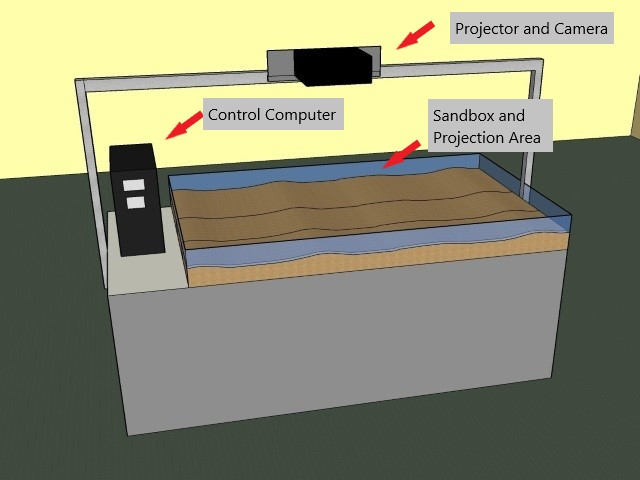
\includegraphics{ARSandbox.jpg}
        \end{center}
    \section{Component Block Diagram}
    \label{ComponentBlockDiagram}
        \begin{center}
        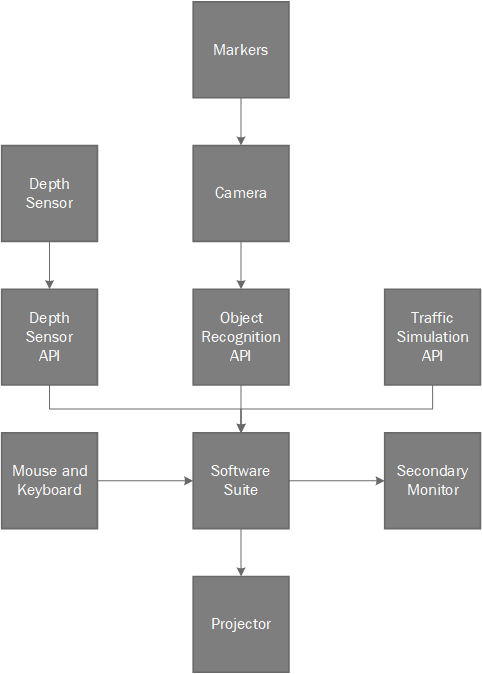
\includegraphics{BlockDiagram.png}
        \end{center}
    \section{Component Flow Diagram}
    \label{ComponentFlowDiagram}
        \begin{center}
        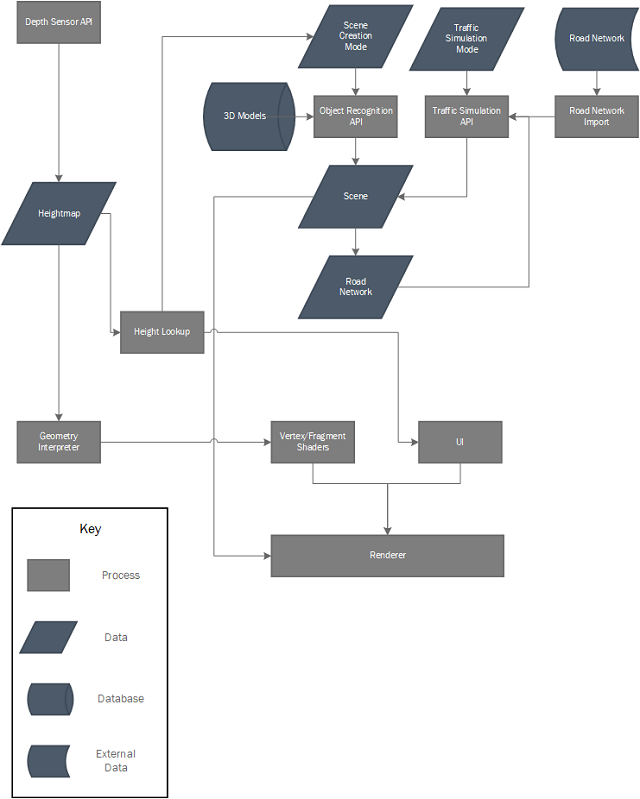
\includegraphics{ComponentFlowDiagram.png}
        \end{center}

%SECTION REFS
\newpage
\bibliographystyle{IEEEtran}
\bibliography{references}
        
\end{document}
